\definecolor{acmGrayFill}{HTML}{B7BDC5}
\definecolor{acmTeal}{HTML}{009E73}
\definecolor{acmBlue}{HTML}{1F77B4}
\definecolor{acmGrid}{HTML}{D9DDE2}
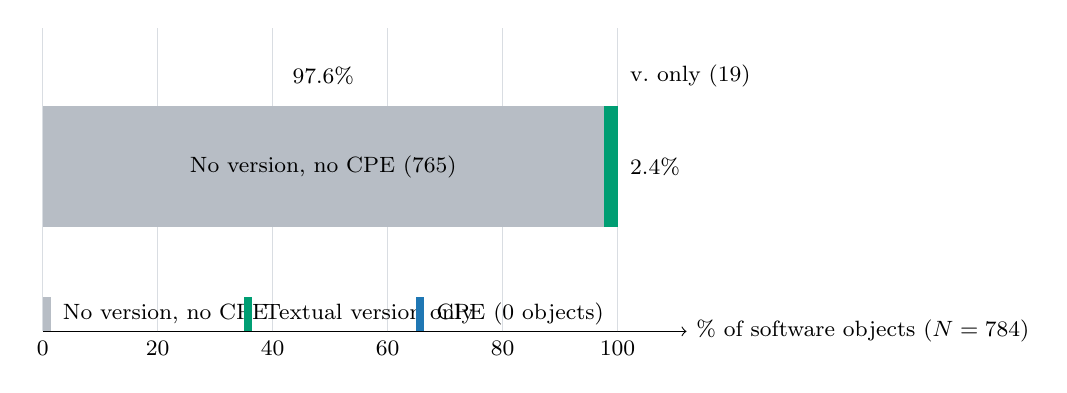
\begin{tikzpicture}[x=0.073cm,y=0.55cm,font=\footnotesize]
  \draw[->] (0,0) -- (112,0) node[right] {\% of software objects ($N=784$)};
  \foreach \x in {0,20,40,60,80,100} {
    \draw[acmGrid] (\x,0) -- (\x,7.0);
    \node[below] at (\x,0) {\x};
  }

  % 97.6 / 2.4 / 0.0 (measured)
  \fill[acmGrayFill] (0,2.4) rectangle (97.6,5.2);
  \fill[acmTeal] (97.6,2.4) rectangle (100,5.2);
  % CPE segment is 0% — no bar

  \node at (48.8,3.8) {No version, no CPE (765)};
  \node[anchor=west] at (100.5,3.8) {2.4\%};

  \node at (48.8,5.9) {97.6\%};
  \node[anchor=west] at (100.5,5.9) {v.~only (19)};

  % Legend
  \fill[acmGrayFill] (0,0.0) rectangle (1.4,0.8);
  \node[anchor=west] at (1.8,0.4) {No version, no CPE};
  \fill[acmTeal] (35,0.0) rectangle (36.4,0.8);
  \node[anchor=west] at (36.8,0.4) {Textual version only};
  \fill[acmBlue] (65,0.0) rectangle (66.4,0.8);
  \node[anchor=west] at (66.8,0.4) {CPE (0 objects)};
\end{tikzpicture}
